\section{Benchmarking the Analysis with Boosted Trees}
Boosted trees have been an essential part of \ac{HEP} analysis for many years (see 
\cite{ATLAS-CONF-2011-152} and \cite{ATLAS-CONF-2017-064}). The XGBoost framework has likewise 
been used as the benchmark for all \ac{ML} analysis, often chosen for its performance in sensitivity and 
extreme \ac{HPC} attributes. Another reason for its popularity is the incredibly simple \ac{API}, allowing 
to create and predict a model in two lines of code. Additionally, its incredible boosting capabilities mean 
that it is little effected by variation in its structure. This leads many to the conclusion that the default 
parameters (see section \ref{subsec:XGBoost}) are often the best. 
\\
I have chosen to run a sensitivity analysis for the original signal data set using a XGBoost model. The results
will act as a benchmark when performing further testing with \ac{NN}-variants. 
\begin{figure}
    \centering
    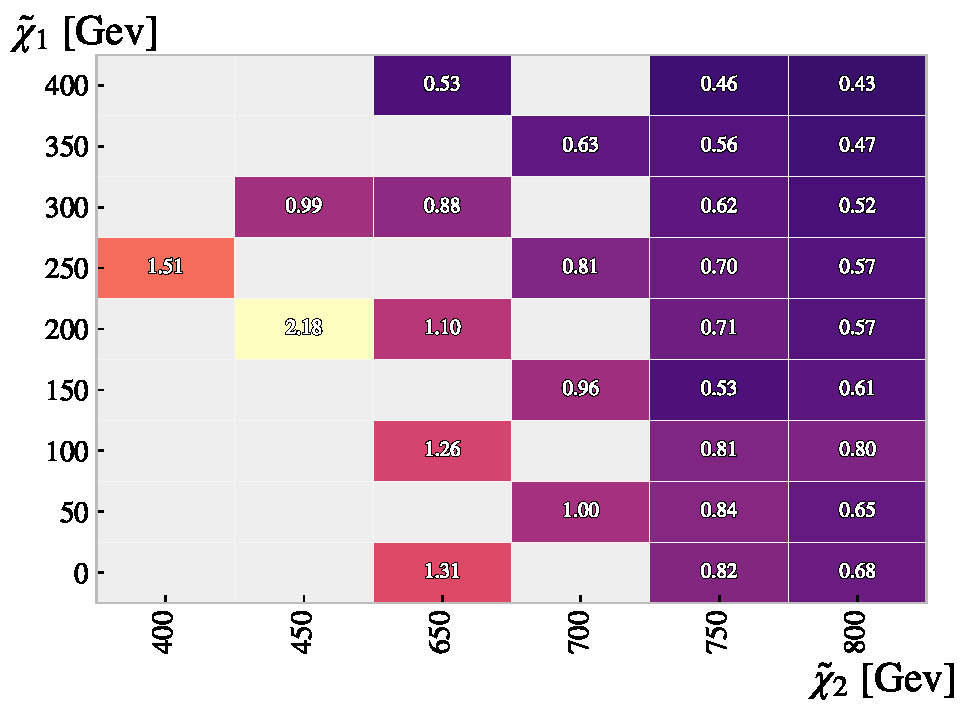
\includegraphics[width=0.7\textwidth]{Figures/MLResults/XGB/SUSY/Grid/XGBGridSig.pdf}
    \caption{A grid displaying the achieved significance on the original signal set, using the signal region 
    created by the \emph{XGBoost} network.}
    \label{fig:XGBoost}
\end{figure}